\RussianSourceFrame{GELFAND-P001435}{10}
\RussianUnclear{GELFAND-P001435}{heading-date}{22.2.88 / 22.2.82}
\underline{Углы между подпространствами.}

\begin{center}
\underline{Серия задач про углы между подпространствами}

(\underline{И.М. Гельфанд}; по записям А.К. Звонкина)
\end{center}

Нек-рые доступны 8-класснику (задачи в $R^2$ и $R^3$),
другие для доктора наук (задачи в гильб. пр-ве).

Что такое «угол» между двумя прямыми на плоскости?
Это ортогональный инвариант этой пары прямых — т.е. некая
числовая хар-ка, к-рая не меняется при всех ортогональных преобр.
плоскости.

Более того, угол — это \underline{полная система инвариантов}, т.е.
пара прямых тогда и только тогда переводится в другую пару
ортог. пр-ем, когда у этих двух пар прямых одинаковый угол.

В дальнейшем под «углом» понимается полная система
инвариантов нек-рого объекта под действием нек-рой группы.
Иногда это число, иногда — конечное или счетное мн-во чисел,
иногда даже континуум чисел.

(В случаях, когда речь будет идти, скажем, о четверке подпр-в
$\Rightarrow$ [стрелка продолжения строки]
лин. пр-ва, не будем употреблять выражение «\underline{угол между\ldots}»,
т.к. непонятно, между чем?, а будем говорить «\underline{угол для\ldots}».)

Во всех задачах представляет интерес не только то,
\underline{что такое угол}, но также и \underline{какие значения он может
принимать}.

\paragraph*{I. \underline{Задачи для школьников.}}
1. Что такое угол между прямой и плоскостью в трёхмерном
пр-ве.

(Два варианта: прямая ориентирована и не ориентирована).

2. Что такое угол между двумя плоскостями в трёхмерном
пространстве?

\paragraph*{II. \underline{Задачи для студентов.}}
3. Дано 4-мерное линейное пр-во со скал. произведением.
(не $R^4$, т.к. не выделены оси). Что такое угол между двумя его
двумерными подпространствами?

4. Дано $\{L,(\cdot,\cdot)\}$, $\dim L=n$, $v\in L$, $V\subset L$,
$\dim V=k$.

Определить угол между $v$ и $V$.


\RussianSourceFrame{GELFAND-P001436}{unlabelled}
5. Дано $\{L,(\cdot,\cdot)\}$, $\dim L=n$, $V,W\subset L$,
$\dim V=k$, $\dim W=m$. Определить угол между $V$ и $W$.

6. Пусть $L$ — просто линейное пространство (без скалярного
произведения). Определить угол для

(а) подпространства $L$

(б) пары подпространств

(в) тройки подпространств.

(Под группой здесь надо понимать $GL(n)$)

7. Дана плоскость Минковского, т.е. $L$, $\dim L=2$
с незнакоопределенным скалярным произведением $-x_1^2+x_2^2$.
Определить угол между двумя прямыми (т.е. инвариант
относительно группы преобразований, сохраняющих это
скалярное произведение).

8. Дальнейшие вариации:
\begin{itemize}
\item[—] для пространства Минковского более высокой размерности
и двух его подпространств
\item[—] для других пространств с неопределенной метрикой
(т.е. когда в скалярном произведении более чем один минус)
\item[—] для пространств с вырожденной формой (например, $R^3$
со скалярным произведением $x_1^2+x_2^2$).
\end{itemize}

Для всех перечисленных задач надо рассмотреть случаи
групп $O(n)$ и $SO(n)$.

\paragraph*{III. \underline{Задачи для аспирантов.}}
9. Дано лин. пр-во $L$ и четверка его подпр-в. Найти угол
этой четверки (это содержание работы Гельфанда и Пономарева)

10. (А.А. Кириллов-младший) Дано $\{L,(\cdot,\cdot)\}$; тогда в тензорных
степенях $L$ тоже определено скалярное произведение. Пусть
$a,b\in L\otimes L$. Найти угол между подпространствами $a\otimes L$ и
$L\otimes b$, вложенными в $L\otimes L\otimes L$.

(Это нужно для алг-р Гекке и ур-я Яна-Бакстера)


\RussianSourceFrame{GELFAND-P001437}{11}
\paragraph*{IV. \underline{Задачи для кандидатов и док-торов наук.}}
11. Определить угол для двух подпр-в гильбертова пр-ва.
Привести примеры, когда значением угла является счётное
мн-во чисел, и когда — континуум чисел.

12. Та же задача для гильбертова пр-ва с неопределенной метрикой.

\paragraph*{\underline{Комментарии.}}
1. В этих задачах особенно трудна вторая часть; например,
если дано подпр-во и угол, а требуется построить
другое подпр-во, лежащее под данным углом к данному.

2. Линейный оператор можно задавать с помощью
четверки подпространств.


\RussianSourceFrame{GELFAND-P001438}{unlabelled}
\underline{21/III-88} \qquad \underline{Сем. Гельфанда}

\underline{\underline{Радул А.}}

\paragraph*{\underline{Квантовые скобки Гельфанда — Дикого}}
(по С. Лукьянову) \qquad Рассм. на $S^1$ оператор
\begin{equation*}
L=\partial_z^N+\sum_{i=0}^{N-1}u_{N-1}(z)\partial_z^i . \tag{1}
\end{equation*}
\RussianUnclear{GELFAND-P001438}{operator-coefficient}{Индекс коэффициента: $N-1$ / $N-i$.}

и пр-во ф-лов вида
\begin{equation*}
f[u]=\oint P\bigl[z,u_i^{(k)}(z)\bigr]dz \tag{2}
\end{equation*}
и их конечных произведений; $P$ — полином по $u_i^{(k)}$.

На таких ф-лах определены 2 скобки Гельфанда — Дикого
\begin{equation*}
\frac{\delta f}{\delta u_i}\quad
\text{опр. из соотн.:}\quad
\left.\frac{d}{d\varepsilon}f[u+\varepsilon\delta u]\right|_{\varepsilon=0}
=\oint dz\,\frac{\delta f}{\delta u_i}\delta u_i . \tag{3}
\end{equation*}

\underline{И.М. Гельфанд}
\paragraph*{\underline{Отступление о функциональном анализе}}
Вся интуиция функц. анализа исходила из того, что ф-лы — это тоже
ф-и, но на $\infty$-мерном пр-ве.

И.М.Г. изменил свою точку зрения и отсюда два следствия.

1) Бывают ф-лы разных типов и их надо классифицировать.

2) Ф-лы — не ф-и $\Rightarrow$ влияет на геометрию.

1) В вар. исчислении бывают ф-лы
\begin{equation*}
\int_0^L f\bigl(x,u(x),u'(x)\bigr)\,dx \tag{*}
\end{equation*}
\RussianUnclear{GELFAND-P001438}{local-functional-argument}{Аргумент среднего $u$: $x$ / $z$.}

Это ф-л от $u$, но он обладает св-вом:

\RussianSourceFigure{GELFAND-P001438}{locality-diagram}{Наклонная линия с двумя выступами вверх; подписи и стрелки не видны. В вершинах выступов есть разрывы штрихов.}

\par\medskip\noindent
\begin{minipage}[c]{0.48\linewidth}\centering
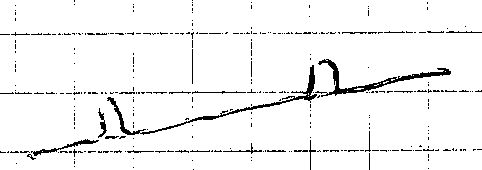
\includegraphics[width=\linewidth]{figures/gelfand-p001438-locality-diagram-original.png}
\par\smallskip{\footnotesize Оригинал рукописного рисунка: GELFAND-P001438\par}
\end{minipage}\hfill
\begin{minipage}[c]{0.48\linewidth}\centering
\resizebox{\linewidth}{!}{% Partial trace of the visible source strokes, in original crop-pixel coordinates.
% No coordinate axes, function values, arrowheads or missing joins are inferred.
\begin{tikzpicture}[x=0.01cm,y=-0.01cm,line width=0.55pt]
\path[use as bounding box] (0,0) rectangle (482,170);
\draw (29,155)--(55,147)--(81,140)--(94,141);
\draw (99,138)--(105,131)--(99,113);
\draw (108,99)--(117,112)--(121,131)--(132,137)
 --(154,132)--(185,121)--(223,113)--(253,108)--(281,102)--(309,96);
\draw (309,96)--(313,87)--(313,66);
\draw (321,62)--(329,61)--(334,68)--(335,88)--(338,94)
 --(356,93)--(380,86)--(404,79)--(426,75)--(446,73);
\draw (441,69)--(449,70)--(451,73);
\end{tikzpicture}
}
\par\smallskip{\footnotesize Частичное воссоздание видимых штрихов; разрывы не соединены.\par}
\end{minipage}\par\medskip


если есть приращ. [вставлено над строкой, со стрелкой к этому месту: $u$]
в 2-х местах, то
приращ. ф-ла (*) будет суммой
[зачеркнуто: \RussianUnclear{GELFAND-P001438}{locality-cancelled}{2 / начало «двух»?}]
приращений

(локальность!)

\underline{\RussianUnclear{GELFAND-P001438}{general-functional-phrase}{5-й возм. обобщ. ф-й: / Б-й возм. обобщ. ф-й:}}
отсюда вытекает
(и из непрерывности),
что тогда [зачеркнуто: \RussianUnclear{GELFAND-P001438}{general-functional-cancelled}{от / он}]
ф-л имеет такой вид

[зачеркнутый знак: \RussianUnclear{GELFAND-P001438}{type-zero-cancelled}{1 / И}]
Это 0-й тип.


\RussianSourceFrame{GELFAND-P001439}{27}
\underline{1-й тип:} если
\begin{equation*}
\frac{\delta}{\delta u}F(u)\quad\text{\underline{локален}.}
\end{equation*}
Таковы ф-лы, встр. в теории Атьи-Зингера

Беда функ. анализа сост. в том, что он \RussianUnclear{GELFAND-P001439}{analysis-verb}{формировался / формулировался / формируется},
когда все [зачеркнуто: \RussianUnclear{GELFAND-P001439}{rationalize-cancelled}{это?}]
\RussianUnclear{GELFAND-P001439}{rationalize-verb}{пытались / пытаешь} рационализировать.

И [зачеркнуто: \RussianUnclear{GELFAND-P001439}{continuity-cancelled}{спектр?}]
в теор. ф-й даже
непрерывность отн. к обл. смерти.

\paragraph*{\underline{Ф-лы:}}
а) длина кривой

б) площадь поверхности \qquad (локальные)

\paragraph*{\underline{Трансценд. ф-лы:}}
(как в анализе — невычисляемые интегралы — эллипт. ф-и)

переход от коэфф. к соб. значениям!!

$\lambda_1$ — такой ф-л.

\underline{Ф-л степ. трансценд. 1} — если вар. производная — лок. ф-л.

и т.д.

\underline{Ф-л [зачеркнуто: \RussianUnclear{GELFAND-P001439}{type-two-cancelled}{ст. / от}]
2-го типа:} если $\dfrac{\delta F}{\delta u}$ — 1-го типа.

Продумывали в раб. Гельфанд, Габриэлов, Лошик,
но заткнулось, т.к. трудно.

В теории [вставлено над строкой: хар.] классов появятся ф-лы всех типов.

Ф-лы надо рассм. на $\infty$-мерных мн-зиях. Но не просто
заменить $n$-мерн. пр-во на $\infty$-мерное!

[зачеркнуто: \RussianUnclear{GELFAND-P001439}{locality-cancelled}{Тут / Род}]
Осн., что локальность играет исключ. роль!

Тогда надо по-другому.

Ф-и образуют алгебру.

Локальные ф-лы не образуют алгебры!!

\underline{Задача:} нужно вариац. исчисление для сумм, произведений
таких ф-лов.


\RussianSourceFrame{GELFAND-P001440}{unlabelled}
\begin{equation*}
\int f\bigl(x,y,u_i(x),u_i'(x),v_i(y),v_i'(y)\bigr)\,dx\,dy
\end{equation*}
Поэтому строить дифф. геом. уже нельзя.

Форм. добавить произведения — плохо!

\underline{\RussianUnclear{GELFAND-P001440}{structures-word}{исход.?}}
структуры, введ. \underline{Г. и Дорфман} и
потом изм. \underline{связность}, \underline{когом. де Рама}, скобки Яна-Бакстера\ldots

\underline{Радул} (продолжение)

Работа: препринт ИПМ; перевод в т. 1 собр. соч.

\paragraph*{\underline{Отступление: символы п.д.о.}}
\begin{equation*}
A=\sum a_i(z)\partial_z^i,\qquad
B=\sum b_j(z)\partial_z^j . \tag{4}
\end{equation*}
\begin{equation*}
\partial_z\longrightarrow\xi
\end{equation*}
\begin{equation*}
AB=\left.A(z,\xi)\circ B(z,\xi)\right|_{\xi=\partial_z}, \tag{5}
\end{equation*}
где
\begin{equation*}
A(z,\xi)\circ B(z,\xi):=
\sum_{n\geq0}\partial_\xi^n A(z,\xi)\,\partial_z^n B(z,\xi)/n!.
\end{equation*}

Переключимся на форм. лорановские ряды:
\begin{equation*}
C(z)[[\xi]]=\left\{\sum_{j=-\infty}^{N}c_i(z)\xi^i\right\}. \tag{6}
\end{equation*}
\RussianUnclear{GELFAND-P001440}{laurent-indices}{Под суммой: $j=-\infty$ / $i=-\infty$; в слагаемом видны индексы $i$.}
\RussianUnclear{GELFAND-P001440}{laurent-argument}{Аргумент $c_i$ переписан: виден $z$ поверх неясного знака ($\xi$ / прежний $z$).}

$\xi^{-1}=\partial_z^{-1}$ обладает
[вставлено над строкой: всеми форм.]
св-ми опер. интегрирования

Операции на символах
\begin{equation*}
\left(\sum_{-\infty}^{N}a_i\xi^i\right)_+
=\sum_{0}^{N}a_i\xi^i \tag{7}
\end{equation*}
\begin{equation*}
\operatorname{res}\left(\sum_{-\infty}^{N}a_i\xi^i\right)=a_{-1} \tag{8}
\end{equation*}

\underline{Градиент $f$.}
\begin{equation*}
\nabla f:=\sum_{j=0}^{N-1}\xi^{-j-1}\circ\frac{\delta f}{\delta u_j}. \tag{9}
\end{equation*}


\RussianSourceFrame{GELFAND-P001441}{28}
Тогда
\begin{equation*}
\delta f=\oint\operatorname{res}\delta L\circ\nabla f \tag{10}
\end{equation*}
здесь $L$ — оператор (1)

1-я скобка (гам. структура)
\begin{equation*}
1\text{ ГС:}\quad \{f,g\}_1=\oint\operatorname{res}[L,\nabla f]\nabla g \tag{11}
\end{equation*}
2-я скобка:
\begin{equation*}
2\text{ ГС:}\quad \{f,g\}_2=
\oint\operatorname{res}\bigl(L(\nabla f L)_+-(L\nabla f)_+L\bigr)\nabla g \tag{12}
\end{equation*}

(13) \underline{Утв.} $\{\quad\}_i$
[зачеркнуто: \RussianUnclear{GELFAND-P001441}{statement-cancelled}{неразборчиво}]
задает на пр-ве ф-лов структуру алгебры Ли.

(14) \underline{Пример.} $N=2$, $u_1=0$, $\partial_z^2+u_2$.

Пусть
\begin{equation*}
u_2(n)=\frac12\,\frac{1}{2\pi i}\oint u_2(z)z^{n+1}\,dz \tag{15}
\end{equation*}
Тогда
\begin{equation*}
\{u_2(n),u_2(m)\}_2=\frac{n^3-n}{12}\delta_{n+m,0}+(n-m)u_2(n+m) \tag{16}
\end{equation*}
(получ. коммут. соотн. алг. Вирасоро!)

(17) \underline{Пример.} $N=3$, $u_1=0$, $\partial_z^3+u_2\partial_z+u_3$.
\begin{equation*}
\{u_2(n),u_2(m)\}_2=\frac{n^3-n}{6}\delta_{n+m,0}+(n-m)u_2(n+m)
\tag*{$(18)_{\text{а}}$}
\end{equation*}
\begin{equation*}
\{u_2(n),u_3(m)\}_2=3(n+1)u_3(m+n)-(m+n+3)u_3(m+n)
\tag*{$(18)_{\text{б}}$}
\end{equation*}
\begin{equation*}
\{u_3(n),u_3(m)\}_2=\ldots+
\sum_{k=-\infty}^{\infty}(m+n-k)u_2(m+n-k)u_2(k)
\tag*{$(18)_{\text{в}}$}
\end{equation*}
(квадрат тензора энергии-импульса)

Далее всюду $\{\quad\}$ означает $\{\quad\}_2$

Вместе это классич. предел какой-то квантовой
\RussianUnclear{GELFAND-P001441}{final-abbreviation}{алг.?} токов.


\RussianSourceFrame{GELFAND-P001442}{unlabelled}
\underline{Мораль.} получается не классич. алгебра Ли, а алгебра с
квадр. соотношениями.

(Хованова Т.)

Дынкин тоже вводил квадр. соотн.

С. Лукьянов заним. квантованием этих скобок.

[Слева под именем: (Сережа)]

(С. Лукьянов — асп. В. Фатеева)

\paragraph*{\underline{Отступление}}
\underline{Преобразование Миуры.} Пусть
\begin{equation*}
L(z)=\partial_z^N+\sum u_{N-i}\partial_z^i
=(\partial_z+v_1)\ldots(\partial_z+v_N) \tag{19}
\end{equation*}
\begin{center}— $\cdot$ —\end{center}
\underline{замеч.} [под пометой: \underline{И.М.Г.}]
Если $(\partial_z+v_1)(\partial_z+v_2)u=f$, то $u$ нах. в квадратурах.

Алг. ур-е в радикалах — теория Галуа

Для дифф. ур-й соотв. теория — теория Пикара-Вессио.

Сейчас этим занимается
[зачеркнуто: \RussianUnclear{GELFAND-P001442}{kolchin-cancelled}{Кол\ldots / Коль\ldots}]
Колчин.
\begin{center}— $\cdot$ —\end{center}
\underline{Р.}

\underline{Разлож.} (19): Миура

\hspace{3em}Купершмидт — Вильсон

\hspace{3em}Дринфельд — Соколов

(20) \underline{Теорема.} Зададим для $v_j$ коммут. соотношения
\begin{equation*}
\{v_i(n),v_j(m)\}=h\delta_{ij}\,n\delta_{m+n,0} \tag{21}
\end{equation*}
(алг. Ли — алг.
\RussianUnclear{GELFAND-P001442}{heisenberg-sign}{$H$ / \#; возможна отмена буквы}
Гейзенберга)

Тогда $u_i$ удовлетворяют алгебр. Г.-Д.
соотнош. (Гельф.-Дикого)

(2-я структура Г.-Д., здесь и ниже)

Получилось, что алг. Ли изоморфна
[зачеркнуто: \RussianUnclear{GELFAND-P001442}{quadratic-cancelled}{квад\ldots / ква\ldots}]
квадр. алгебре, не являющейся алгеброй Ли.

Пусть теперь
\begin{equation*}
L(z)=:(\partial_z+v_1)\ldots(\partial_z+v_N): \tag{22}
\end{equation*}
Какие соотношения?

Введем


\RussianSourceFrame{GELFAND-P001443}{29}
\begin{equation*}
M_0=\operatorname{Hol}\bigl((\mathbb C\backslash0)_z\times
(\mathbb C\backslash0)_w\longrightarrow\mathbb C\bigr)
\end{equation*}
[Под $\operatorname{Hol}$: гол. отобр.]
\begin{equation*}
M=\operatorname{Hol}\bigl(((\mathbb C\backslash0)_z\times
(\mathbb C\backslash0)_w\backslash\Delta)\longrightarrow U(v_1,\ldots,v_N)\bigr)
\end{equation*}
[К $U$ проведена черта от пояснения: универ. оберт. алгебра
алгебры Гейзенберга.]

Элемент $M$ — операторнозначная ф-я.

Рассм. еще оператор
\begin{equation*}
r=\frac{\nu}{2}\ln(z-w)^2\sigma,\qquad \sigma f(z,w)=f(w,z).
\end{equation*}
на ф-ях 2-х переменных

\RussianUnclear{GELFAND-P001443}{operator-letter}{Обозначение оператора: $r$ / $\tau$; тот же знак в (23).}

Тогда если $\nu(\nu-1)=h$, то
\begin{equation*}
\exp(-r)L(z)L(w)\exp r\,[f]=\underline{\underline{O}}(1)
\quad\text{при }z\longrightarrow w \tag{23}
\end{equation*}
\begin{equation*}
\forall f\in M_0
\end{equation*}
\RussianUnclear{GELFAND-P001443}{boundedness-symbol}{Знак перед $(1)$ обведен и дважды подчеркнут: $O$ / $0$; возможен прежний знак под обводкой.}

Это набор соотношений на $u_i$ (на коэффициенты)

Результат:
\begin{equation*}
[u_i(z),u_j(w)]=
\left[\sum_{k\geq2}(z-w)^{-k}
\sum_{p+q=i+j-k}c_{ij}^{pq}(k)[u_p(z),u_q(w)]\right] \tag{24}
\end{equation*}
[К правой внешней скобке направлена снизу стрелка от надписи:
«$+$ или $-$».]

$c_{ij}^{pq}(k)$ выраж. через гипергеометрич. ф-и, но сложно

Форма [под словом: \RussianUnclear{GELFAND-P001443}{formula-subline}{скобки.?}]
(23) похожа на соотн. в квант. методе обр. задачи.
\begin{equation*}
L(z)L(w)=R^{-1}L(w)L(z)R. \tag{25}
\end{equation*}


\RussianSourceFrame{GELFAND-P001444}{unlabelled}
\paragraph*{\underline{\underline{М. Капранов.}}}
\underline{Представления колчанов и производная категория.}

(\underline{О раб. \RussianUnclear{GELFAND-P001444}{reference-name}{Партасарати / Парнасарати}
о предст. колчанов.})

\underline{Колчан} — ориент. граф без циклов

\begin{center}
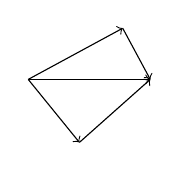
\begin{tikzpicture}
\draw[->] (0,0) -- (1.2,0.65);
\draw[->] (1.2,0.65) -- (1.55,0);
\draw[->] (0,0) -- (1.55,0);
\draw[->] (0,0) -- (0.65,-0.8);
\draw[->] (0.65,-0.8) -- (1.55,0);
\end{tikzpicture}
\end{center}
$\Lambda$ — граф

$\Omega$ — ориентация

$M(\Lambda,\Omega)$ —
[зачеркнуто: \RussianUnclear{GELFAND-P001444}{category-cancelled}{пр\ldots / кат\ldots}]
категория представлений колчана

$\mathcal D(\Lambda,\Omega)$ — производная категория этой категории.

(1) \underline{Лемма.}

Тогда $\mathcal D(\Lambda,\Omega)$ не зависит от $\Omega$

($\mathcal D(\Lambda,\Omega_1)$ и $\mathcal D(\Lambda,\Omega_2)$ эквивалентны)

при разных $\Omega_1$ и $\Omega_2$

\underline{Д-во:} применение симметрии.

\underline{Задача:} найти такие
[зачеркнуто: \RussianUnclear{GELFAND-P001444}{derived-cancelled}{$\mathcal D^{\ell}(\mathcal A)$ / $\mathcal D^{e}(\mathcal A)$ / $\mathcal D^{b}(\mathcal A)$}]
подкатегории $\mathcal A\subset\mathcal D(\Lambda,\Omega)$,
что
\begin{equation*}
\mathcal D^{\ell}(\mathcal A)=\mathcal D(\Lambda,\Omega)
\end{equation*}
\RussianUnclear{GELFAND-P001444}{subcategory-sign}{Знак между $\mathcal A$ и $\mathcal D(\Lambda,\Omega)$ обведен: $\subset$; внутри виден угловой знак $<$ / прежняя черта.}
\RussianUnclear{GELFAND-P001444}{derived-exponent}{Верхний индекс при $\mathcal D$: $\ell$ / $e$ / $b$.}

Все они найдены и характериз. графами Дынкина.

Используются отражения и склейки (и идеология извращенных пучков)

\underline{Замеч. ИМГ}
Классифик. вект. рассл. на $CP^n$ делается только на языке
производных категорий.

\underline{Гротендик:} тяжелым трудом добыл понятия, ведущие к производной категории
(как Микеланджело).

\underline{\underline{М.К.}}

\RussianSourceFigure{GELFAND-P001444}{reflection-quiver}{Слева колчан с четырьмя вершинами: $V_\alpha$ слева, $V_\beta$ сверху, $V_\gamma$ справа, нижняя вершина без подписи. Стрелки идут слева к верхней, правой и нижней вершинам; от верхней и нижней — к правой. Над ребром $V_\alpha\to V_\beta$ стоит $f$; над горизонтальным ребром имеется обведенный или отмененный знак, неуверенно читаемый как $g$ / $\varphi$. Подпись этого ребра требует сверки с оригиналом.}

\par\medskip\noindent
\begin{minipage}[c]{0.48\linewidth}\centering
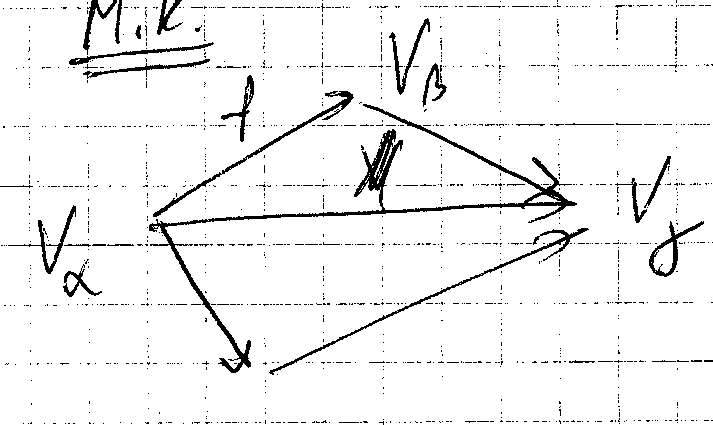
\includegraphics[width=\linewidth]{figures/gelfand-p001444-reflection-quiver-original.png}
\par\smallskip{\footnotesize Оригинал рукописного рисунка: GELFAND-P001444\par}
\end{minipage}\hfill
\begin{minipage}[c]{0.48\linewidth}\centering
\resizebox{\linewidth}{!}{% Partial recreation of five visible directed edges and readable vertex labels.
% The lower vertex is unlabelled in the source. The bracketed edge label is uncertain.
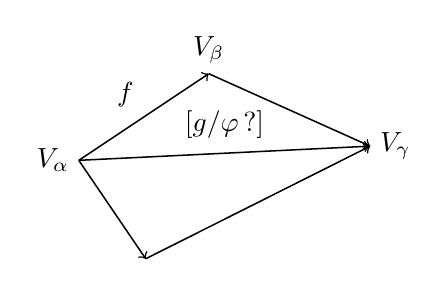
\begin{tikzpicture}[line width=0.55pt]
\coordinate (a) at (0,0);
\coordinate (b) at (1.65,1.10);
\coordinate (c) at (3.70,0.18);
\coordinate (d) at (0.85,-1.25);
\draw[->] (a)--node[above left]{$f$}(b);
\draw[->] (b)--(c);
\draw[->] (a)--(c);
\draw[->] (a)--(d);
\draw[->] (d)--(c);
\node[left] at (a) {$V_\alpha$};
\node[above] at (b) {$V_\beta$};
\node[right] at (c) {$V_\gamma$};
\node[above] at (1.85,0.15) {$[g/\varphi\,?]$};
\end{tikzpicture}
}
\par\smallskip{\footnotesize Частичное воссоздание; в скобках даны неуверенные кандидаты подписи ребра, возможно зачёркнутой.\par}
\end{minipage}\par\medskip


\underline{Отражение} а) $s_\alpha\Omega$ — обращаем стрелки,
исходящие из $\alpha$.

б)
\begin{equation*}
(s_\alpha V)_{\beta\ne\alpha}=V_\beta
\end{equation*}
\begin{equation*}
(s_\alpha V)_\alpha=\bigoplus_{\alpha\to\beta}V_\beta/(\text{образу }V_\alpha)
\end{equation*}
с соотв. отображениями

Могут быть векторы из $V_\alpha$, к-рые всюду переходят в $0$

\begin{center}
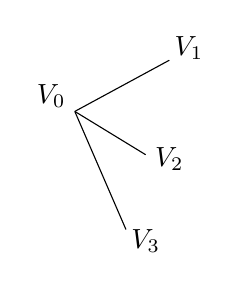
\begin{tikzpicture}
\node at (-0.3,0.2) {$V_0$};
\draw (0,0) -- (1.2,0.65);
\draw (0,0) -- (0.9,-0.55);
\draw (0,0) -- (0.65,-1.5);
\node at (1.45,0.8) {$V_1$};
\node at (1.2,-0.6) {$V_2$};
\node at (0.9,-1.65) {$V_3$};
\end{tikzpicture}
\end{center}
\begin{equation*}
V_0\longrightarrow V_1\oplus V_2\oplus V_3
\end{equation*}

